%%
%% Copyright 2007, 2008, 2009 Elsevier Ltd
%%
%% This file is part of the 'Elsarticle Bundle'.
%% ---------------------------------------------
%%
%% It may be distributed under the conditions of the LaTeX Project Public
%% License, either version 1.2 of this license or (at your option) any
%% later version.  The latest version of this license is in
%%    http://www.latex-project.org/lppl.txt
%% and version 1.2 or later is part of all distributions of LaTeX
%% version 1999/12/01 or later.
%%
%% The list of all files belonging to the 'Elsarticle Bundle' is
%% given in the file `manifest.txt'.
%%

%% Template article for Elsevier's document class `elsarticle'
%% with harvard style bibliographic references
%% SP 2008/03/01
%%
%%
%%
%% $Id: elsarticle-template-harv.tex 4 2009-10-24 08:22:58Z rishi $
%%
%%
%%\documentclass[preprint,authoryear,12pt]{elsarticle}

%% Use the option review to obtain double line spacing
\documentclass[authoryear,preprint,review,12pt]{elsarticle}

%% Use the options 1p,twocolumn; 3p; 3p,twocolumn; 5p; or 5p,twocolumn
%% for a journal layout:
%% \documentclass[final,authoryear,1p,times]{elsarticle}
%% \documentclass[final,authoryear,1p,times,twocolumn]{elsarticle}
%% \documentclass[final,authoryear,3p,times]{elsarticle}
%% \documentclass[final,authoryear,3p,times,twocolumn]{elsarticle}
%% \documentclass[final,authoryear,5p,times]{elsarticle}
%% \documentclass[final,authoryear,5p,times,twocolumn]{elsarticle}

%% if you use PostScript figures in your article
%% use the graphics package for simple commands
\usepackage{graphics}
\usepackage{longtable}
%% or use the graphicx package for more complicated commands
%% \usepackage{graphicx}
%% or use the epsfig package if you prefer to use the old commands
%% \usepackage{epsfig}

%% The amssymb package provides various useful mathematical symbols
\usepackage{amssymb}
%% The amsthm package provides extended theorem environments
\usepackage{amsthm}
\usepackage{colortbl}

%% The lineno packages adds line numbers. Start line numbering with
%% \begin{linenumbers}, end it with \end{linenumbers}. Or switch it on
%% for the whole article with \linenumbers after \end{frontmatter}.
%% \usepackage{lineno}

%% natbib.sty is loaded by default. However, natbib options can be
%% provided with \biboptions{...} command. Following options are
%% valid:

%%   round  -  round parentheses are used (default)
%%   square -  square brackets are used   [option]
%%   curly  -  curly braces are used      {option}
%%   angle  -  angle brackets are used    <option>
%%   semicolon  -  multiple citations separated by semi-colon (default)
%%   colon  - same as semicolon, an earlier confusion
%%   comma  -  separated by comma
%%   authoryear - selects author-year citations (default)
%%   numbers-  selects numerical citations
%%   super  -  numerical citations as superscripts
%%   sort   -  sorts multiple citations according to order in ref. list
%%   sort&compress   -  like sort, but also compresses numerical citations
%%   compress - compresses without sorting
%%   longnamesfirst  -  makes first citation full author list
%%
%% \biboptions{longnamesfirst,comma}

% \biboptions{}

\journal{Expert Systems with Applications}

\newtheorem{definition}{Definition}
\newtheorem{proposition}{Proposition}

\begin{document}

\begin{frontmatter}

%% Title, authors and addresses

%% use the tnoteref command within \title for footnotes;
%% use the tnotetext command for the associated footnote;
%% use the fnref command within \author or \address for footnotes;
%% use the fntext command for the associated footnote;
%% use the corref command within \author for corresponding author footnotes;
%% use the cortext command for the associated footnote;
%% use the ead command for the email address,
%% and the form \ead[url] for the home page:
%%
%% \title{Title\tnoteref{label1}}
%% \tnotetext[label1]{}
%% \author{Name\corref{cor1}\fnref{label2}}
%% \ead{email address}
%% \ead[url]{home page}
%% \fntext[label2]{}
%% \cortext[cor1]{}
%% \address{Address\fnref{label3}}
%% \fntext[label3]{}

\title{Hardware-Software Platform for Computing Irreducible Testors}

%% use optional labels to link authors explicitly to addresses:
%% \author[label1,label2]{<author name>}
%% \address[label1]{<address>}
%% \address[label2]{<address>}

\author{Vlad\'imir Rodr\'iguez}
\author{Ren\'e Cumplido}
\author{J. Ariel Carrasco-Ochoa}
\author{Claudia Feregrino}
\author{J. Francisco Mart\'inez-Trinidad}

\address{Computer Science Department}
\address{National Institute for Astrophysics, Optics and Electronics}
\address{Sta. Ma. Tonanzintla, Puebla, 72840, Mexico}

\begin{abstract}
In pattern recognition, feature selection is a very important task
for supervised classification. The problem consists in, given a
dataset where each object is described by a set of features, finding
a subset of the original features such that a classifier that runs
on data containing only these features would reach high
classification accuracy. A useful way to find this subset of the
original features is through Testor Theory. A testor is defined as a
subset of the original features that allows differentiating objects
from different classes. Testors are very useful particularly when
object descriptions contain both numeric and non-numeric features.
Computing testors for feature selection is a very complex problem
due to exponential complexity, with respect to the number of
features, of algorithms based on testor theory. Hardware
implementation of testor computing algorithms helps to improve their
performance taking advantage of parallel processing for verifying if
a feature subset is a testor in a single clock cycle. This paper
introduces an efficient hardware-software platform for computing
irreducible testors for feature selection in pattern recognition.
Results of implementing the proposed platform using a FPGA-based
prototyping board are presented and discussed.

\end{abstract}

\begin{keyword}
%% keywords here, in the form: keyword \sep keyword
Feature Selection \sep Testor Theory \sep Custom Architectures \sep
FPGAs
%% MSC codes here, in the form: \MSC code \sep code
%% or \MSC[2008] code \sep code (2000 is the default)

\end{keyword}

\end{frontmatter}

% \linenumbers

%% main text
\section{Introduction}
\label{sect:1}

Reconfigurable computing based on the combination of conventional
microprocessors and field programmable gate arrays (FPGAs), has
become increasingly popular for implementing special-purpose
hardware to accelerate complex tasks. Usually an FPGA-based
implementation is embedded in a PC or workstation, which drives its
activity and manages the results. Following this trend, we developed
an efficient hardware-software platform for computing irreducible
testors \citep{R1} for feature selection in pattern recognition
\citep{R2,R3,R17,R18,R19}.

The feature selection problem in pattern recognition consists in,
given a dataset where each object is described by a set of features,
finding a subset of the original features such that a classifier
that runs on data containing only these features would reach higher
classification accuracy. This procedure can reduce not only the cost
of recognition by reducing the number of features to be collected,
but in some cases it can also provide better classification
accuracy. For this task, a higher performance with lower
computational effort is expected \citep{R2}. Several algorithms have
been proposed for feature selection, however, most of them were
developed for numeric features \citep{R3,R4}. 
% adecuate these sentences %%%%%%%%%%%%%%%%%%%%%%%%%%%%%%%%%%%%%%%%%%
We chose CT-EXT, an algorithm based on testor theory, which can be applied on datasets
described with both numeric and non-numeric features, even when
there are missing data. Although the theoretical aspect of computing
irreducible testors is advanced \citep{R5,R6,R7,R8,R9}, there are
not practical hardware implementations reported previously,
excepting our previous works.
%%%%%%%%%%%%%%%%%%%%%%%%%%%%%%%%%%%%%%%%%%%%%%%%%%%%%%%%%%%%%%%%%%%%%%%%%%
% add news improvements and correct some sentences %%%%%%%%%%%%%%%%%%%%%%%%%%%%%%%%%%%%%%%%%%%%%%%%%%%%%%%
In our first work, an architectural design based on a brute force approach for computing testors was proposed
\citep{R10}. In this first approach, each candidate was generated by a counter that incremented its value by
1 on each iteration. The architecture is able to evaluate if a candidate is a testor in a single clock cycle,
however, the architecture did not exploit the characteristics of a particular data set that could allow to
significantly reduce the number of candidates tested.  The next step in our architectural design \citep{R11}
was the implementation of BT algorithm for computing testors where a candidate generator that jumps over
unnecessary candidates allows reducing the number of comparisons needed in the brute force approach. These
two previous works compute the whole set of testors, however for pattern recognition applications where
testor theory can be applied, it is important to obtain only testors that are irreducible. Thus, as the next step in our design, in \citep{R21} we proposed a hardware-software platform for computing only irreducible testors.
This platform consisted of the combination of a specialized hardware architecture that was implemented on a
commercial FPGA-based prototyping board and a host application running on a PC. The architecture implemented
the BT algorithm, as in \citep{R11}, but it also included a new module that eliminates most of the testors
that are not irreducible before transferring them to the host application for final processing.
In this work we present an architecture that implements the CT-EXT algorithm and is capable of finding only irreducible testors. The CT-EXT algorithm has proven more efficient in finding typical testors than BT algorithm in most cases \citep{R22, R23}.
%%%%%%%%%%%%%%%%%%%%%%%%%%%%%%%%%%%%%%%%%%%%%%%%%%%%%%%%%%%%%%%%%%%%%%%%%%%%%%%%%%%%%%%%%%%%%%%%%%%%%%%%%%%%
The intensive computational requirements due to the exponential
complexity, with respect to the number of features, of the testor
theory based algorithms can be met by a combination of technological
improvements and efficient hardware architectures based on parallel
computational models. Specific parallel architectures can be
designed to exploit the parallelism found in the irreducible testor
computing algorithms. Further optimizations such as incremental
processing and the use of multiple processing elements are also
possible.

\section{Basic concepts}
\label{sect:2}

In pattern recognition, feature selection is a very important task for supervised classification. A useful
way to do this selection is through Testor Theory. The concept of testor for pattern recognition was
introduced by Dmitriev et al. in 1966 \citep{R12}. They defined a testor as a subset of features that allows
differentiating objects from different classes. Testors are quite useful, especially when object descriptions
contain both numeric and nonnumeric features, and maybe they are incomplete (mixed incomplete data)
\citep{R5}.

Let $TM$ be a training matrix with $K$ objects described through $N$
features of any type $(x_{1},\ldots,x_{N})$ and grouped in $r$
classes. Let $DM$ be a dissimilarity Boolean matrix (0 = similar,1 =
dissimilar), obtained from feature by feature comparisons of every
pair of objects from $TM$ belonging to different classes. $DM$ has
$N$ columns and $M$ rows, where $M>>K$.

Testors and irreducible testors are defined as follows:

\begin{definition} \label{def1}
A subset of features $T$ is a testor if and only if when all
features are eliminated from $DM$, except those from $T$, there is
not any row of $DM$ with only 0�s.
\end{definition}


\begin{definition} \label{def2}
A subset of features $T$ is an irreducible testor if and only if $T$
is a testor and there is not any other testor $T'$ such that
$T'\subset T$.
\end{definition}

In defintion \ref{def1}, if there is not any row of $DM$ with only
0's it means that there is not a pair of objects from different
classes that are similar on all the features of $T$, that is, a
testor $T$ allows differentiating between objects from different
classes.

The number of rows in $DM$ could be too large, therefore a strategy to reduce this matrix without losing
relevant information for computing irreducible testors was introduced by Lazo et al \citep{R1}.

\begin{definition} \label{def3}
If $t$ and $p$ are two rows of $DM$, then $p$ is a sub-row of $t$ if and only if:


\begin{enumerate}
\renewcommand{\labelenumi}{\alph{enumi})}
\item $t$ has 1 everywhere $p$ has 1
\item there is at least one column such that $t$ has 1 and $p$ has 0
\end{enumerate}
\end{definition}

\begin{definition} \label{def4}
A row $t$ of $DM$ is a basic row of $DM$ if and only if $DM$ does
not have any other row $t' $ such that $t' $ is a sub-row of $t$.
\end{definition}

\begin{definition} \label{def5}
The matrix that contains only the basic rows of $DM$ is called basic
matrix and is denoted by $BM$.
\end{definition}

Let $TT(M)$ be the set of all irreducible testors of the Boolean matrix M, then

\begin{proposition}
$TT(DM)=TT(BM)$.
\end{proposition}

This proposition indicates that the set of all irreducible testors calculated using $DM$ or $BM$ is the same
\citep{R1}. However, $BM$ is smaller than $DM$ and the construction of $BM$ from $DM$ is a very fast process,
for example, the time for obtaining a $BM$ matrix with 48 columns and 32 rows from a $DM$ matrix with 48
columns and 193,753 rows, is about 0.21 seconds on a PC with an Intel Centrino Duo processor running at
1.6GHz, with 1024 MB of RAM.

The CT-EXT has the following theoretical bases.
\begin{definition} \label{def21} Let $f_i$ be a row of BM. We say that $f_i$ is a zero row of $S \subseteq R$, and we denote it by ${f_i}^0 (S)$, if $\forall X_p \in S$, $f_i [p] = BM [i, p] = 0$.
\end{definition}
\begin{definition} \label{def22} In terms of BM, a testor $T \subseteq R$ is a feature set such that there
are no zero rows of T in BM. 
\end{definition}
From this definition, if T is a testor then, any superset of T is a testor too.
\begin{definition} \label{def23} Let $f_i$ be a row of BM. We say that $f_i$ is a typical (irreducible) row of $S \subseteq R$ with regard to $X_q$ , and we denote it by ${f_i}^1 (S,q)$ if $\exists X_q \in S$, such that $f_i [q] = BM [i, q] = 1$, and $\forall X_p \in S$, $X_p \neq X_q$ , $f_i [p] = BM [i, p] =~0$.
\end{definition}

\begin{definition} \label{def24} In terms of BM, $T \subseteq R$ is a typical testor if T is a testor and
$\forall X_j \in T, \exists {f_i}^1 (T, j)$.
\end{definition}

This means that in a typical testor, for all features, there exists a row in BM in
the sub matrix associated to T, having a value of 1 in the position corresponding
to that feature, and values of 0 in all remaining positions (there are no zero rows,
and if any column of T is eliminated, at least one zero row appears, and the testor
property is not fulfilled). Although we have defined a typical testor here in terms
of BM, normally it is defined as an irreducible testor (as in definition~\ref{def2}).

\begin{definition} \label{def25} Let $T \subseteq R$ and $X_j \in R$, $X_j \neq T$. We denote by
$\sum_T f^0$ the number of zero rows of T. We say that $X_j$ contributes to T if, and only if,
$\sum_{T\cup\{X_j\}} f^0 < \sum_T f^0$.
\end{definition}
This definition indicates that one feature contributes to a feature combination
if for some zero rows in BM, considering only T, the new feature has a value of
1 in at least one of these zero rows. So, adding this feature to T, there are less
zero rows of the incremented feature combination than of T.

Being $T \subset T\cup\{X_j\}$, it is not possible that $\sum_T f^0 < \sum_{T\cup\{X_j\}} f^0$. If we
increase the feature combination either the zero rows are maintained and in this
case the column added does not contribute to the combination, or the number of zero rows decreases.

\begin{proposition}\label{prop1} Let $T \subseteq R$ and  $X_j \in R$, $X_j \neq T$. If $X_j$ does not contribute to
T, then $T\cup\{X_j\}$ can not generate any typical testor.
\end{proposition}

\textit{Proof}. Let $T \subseteq R$ and $X_j \in R$, such that $X_j$ does not contribute to T. Suppose
that $T' = T\cup\{X_j \cup Z\}$ is a typical testor. Then, according to definition \ref{def24}, there
exists for $X_j$ at least a typical row in BM. Then, $f_i [j] = BM [i, j] = 1$, and
$\forall X_p \in T'$ , $X_p \neq X_j$ , $f_i [p] = BM [i, p] = 0$. Thus, we have that $f_i$ is a zero row
of $T \cup Z$ and therefore, of T too. So, $\sum_{T\cup\{X_j\}} f^0 < \sum_T f^0$ and we obtain that
$X_j$ contributes to T, which contradicts the formulated hypothesis and then, we
have that there are no typical testors that include $T\cup\{X_j\}$.

\begin{proposition}\label{prop2} Let $T \subseteq R$, $Z \subseteq R$, $Z \neq \emptyset$. If T is a testor, then $T \cup Z$ is a testor too, but it is not a typical testor.
\end{proposition}

\textit{Proof}. Being T a testor, we have that $\sum_T f^0 = 0$, therefore, any feature $X_p \in Z$
contributes to T. Since $T \cup Z$ is a superset of T, then $T \cup Z$ is a testor, but
following proposition~\ref{prop1}, it can not generate any typical testor.
\subsection*{Description of the CT-EXT algorithm}
%\texttt{
%\textbf{Input:} BM (Basic Matrix)\\
%\textbf{Output:} TT (set of all typical testors)}
\begin{enumerate}
\item The row with less quantity of 1's, is set as the first row of BM. The columns of BM are ordered, from left to right, each having a value of 1 in the first row and each subsequent column having a value 0 in the first row of BM. The order of the columns into each group (with the same value of 1 or with the same value of 0) is irrelevant.

\item Let the set TT = \{~\} (initialized as empty set, it will be the typical testors set) and the list T = [~]  (current feature combination); j = 1 (first feature of BM to be analyzed).

\item If $X_j$ has a value of 1 in the first row of BM then $X_j$ is added to T $(T = T [X_j])$, go to
step 5; otherwise, the algorithm finishes (any new feature combination
will not generate a typical testor, because all these combinations have a zero row).
The new feature is added to the current

\item The new feature is added to the current combination ($T = T \cup \{X_j\}$), and it is verified whether this new feature contributes to the current combination. If the answer is negative, go to step 6.

\item Verify whether T is a testor, if yes then verify whether it is a typical testor. If T is a typical testor, the combination is saved in TT ($TT = TT \cup T $). If this is not the case, go to step 7.

\item The last feature analysed $X_j$ is eliminated from T ($T = T \setminus \{Xj\}$). If $X_j$ does not contribute
to T, then no combination containing T is verified (proposition \ref{prop1}). Go to step 7. If the
 combination was a testor, then no consecutive superset of the current combination is analysed 
 (proposition \ref{prop2}). If $T = \emptyset$ then $j = j + 1$, go to step 3.
 
\item The next non-analysed feature in the current combination is selected. If $j < n$ then $j = j + 1$, 
and go to step 4; otherwise, go to step 6.
\end{enumerate}

For example consider the basic matrix of Table~\ref{table1}, with N=5 attributes and M=3 rows. After ordering step we obtain the basic matrix of Table~\ref{table2}. Table~\ref{tab_example} illustrates solution process.

\begin{table}[!htb]
    \begin{minipage}{.5\linewidth}
      \caption{Basic Matrix for the example.}\label{table1}
      \centering
        \begin{tabular}{ ccccc }
 			\hline                       
  			$x_0$ & $x_1$ & $x_2$ & $x_3$ & $x_4$ \\
  			\hline
  			1 & 0 & 0 & 1 & 1 \\
  			0 & 1 & 1 & 0 & 1 \\
  			1 & 1 & 0 & 0 & 1 \\
  			\hline  
		\end{tabular}
    \end{minipage}%
    \begin{minipage}{.5\linewidth}
      \centering
        \caption{Ordered Basic Matrix.}\label{table2}
        \begin{tabular}{ ccccc }
 			\hline                       
  			$x_0$ & $x_3$ & $x_4$ & $x_1$ & $x_2$ \\
  			\hline
  			1 & 1 & 1 & 0 & 0 \\
  			0 & 0 & 1 & 1 & 1 \\
  			1 & 0 & 1 & 1 & 0 \\
  			\hline  
		\end{tabular}
    \end{minipage} 
\end{table}

\newcommand{\lcell}[2][2.5in]{$\vcenter{\hsize#1\baselineskip11pt\vspace*{3.5pt}\raggedright#2\strut\par}$}

      %\centering
        \begin{longtable}{cccccl}
		\caption[CT-EXT example.]{CT-EXT algorithm example.} \label{tab_example} \\
 			\hline                       
  			$\mathbf{T}$ & $\mathbf{\sum_T f^0}$ & $\mathbf{X_j}$ & $\mathbf{T \cup \{X_j\}}$ &
  			$\mathbf{\sum_{T \cup \{X_j\}} f^0}$ & 
  			\multicolumn{1}{>{\centering\arraybackslash}m{2.5in}}{\textbf{Comments}}\\
  			\hline
  			$\{~\}$ & $\infty$ & $x_0$ & $\mathbf{\{x_0\}}$ & 1 & 
  			\lcell{$x_0$ contributes but $\{x_0\}$ isn't a testor. Add a new attribute (step~7).}\\
  			$\{x_0\}$ & 1 & $x_3$ & $\mathbf{\{x_0,x_3\}}$ & 1 &
  			\lcell{$x_3$ doesn't contributes. Eliminate $x_3$ (step 6). Add a new attribute.}\\
  			$\{x_0\}$ & 1 & $x_4$ & $\mathbf{\{x_0,x_4\}}$ & 0 &
  			\lcell{$x_4$ contributes, $\{x_0,x_4\}$ is testor but isn't irreducible.
  			 	Eliminate $x_4$. Add a new attribute.}\\
  			$\{x_0\}$ & 1 & $x_1$ & $\mathbf{\{x_0,x_1\}}$ & 0 &
  			\lcell{$x_1$ contributes, $\{x_0,x_1\}$ is an irreducible testor.
  				It is saved ($TT = \{\{x_0,x_1\}\}$).
  			 	Eliminate $x_1$. Add a new attribute.}\\
  			$\{x_0\}$ & 1 & $x_2$ & $\mathbf{\{x_0,x_2\}}$ & 0 &
  			\lcell{$x_2$ contributes, $\{x_0,x_1\}$ is an irreducible testor.
  				It is saved ($TT = \{\{x_0,x_1\},\{x_0,x_2\}\}$).
  			 	Eliminate $x_1$. Add a new attribute.}\\
  			$\{x_0\}$ & \multicolumn{5}{>{\centering\arraybackslash}m{5in}}{All attributes tested. 
  			Eliminate $x_0$ and add a new one (step 3).}\\
  			\hline 
  			$\{~\}$ & $\infty$ & $x_3$ & $\mathbf{\{x_3\}}$ & 2 & 
  			\lcell{$x_3$ contributes but $\{x_3\}$ isn't a testor. Add a new attribute.}\\
  			$\{x_3\}$ & 2 & $x_4$ & $\mathbf{\{x_3,x_4\}}$ & 0 &
  			\lcell{$x_4$ contributes, $\{x_3,x_4\}$ is testor but isn't irreducible.
  			 	Eliminate $x_4$. Add a new attribute.}\\
  			$\{x_3\}$ & 2 & $x_1$ & $\mathbf{\{x_3,x_1\}}$ & 0 &
  			\lcell{$x_1$ contributes, $\{x_3,x_1\}$ is an irreducible testor.
  				It is saved ($TT = \{\{x_0,x_1\},\{x_0,x_2\},\{x_3,x_1\}\}$).
  			 	Eliminate $x_1$. Add a new attribute.}\\
  			$\{x_3\}$ & 2 & $x_2$ & $\mathbf{\{x_3,x_2\}}$ & 1 & 
  			\lcell{$x_2$ contributes but $\{x_3,x_2\}$ isn't a testor. Add a new attribute.}\\
  			$\{x_3\}$ & \multicolumn{5}{>{\centering\arraybackslash}m{5in}}{All attributes tested. 
  			Eliminate $x_3$ and add a new one (step 3).}\\
  			\hline 
  			$\{~\}$ & $\infty$ & $x_4$ & $\mathbf{\{x_4\}}$ & 0 & 
  			\lcell{$x_4$ contributes, $\{x_4\}$ is an irreducible testor.
  				It is saved ($TT = \{\{x_0,x_1\},\{x_0,x_2\},\{x_3,x_1\},\{x_4\}\}$).
  			 	Eliminate $x_4$. Add a new attribute (step 3).}\\
  			\hline  
  			$\{~\}$ & $\infty$ &  $\mathbf{\{x_1\}}$ & \multicolumn{3}{>{\centering\arraybackslash}m{4in}}{
  			$x_1$ has value '0' in first row of BM, Algorithm is done.}\\
  			\hline  
		\end{longtable}

\section{Proposed platform}
\label{sect:3}

Since algorithms for computing all irreducible testors have
exponential complexity, with respect to the number of columns in
$BM$, software based implementations do not provide reasonable
performance for practical problems. An interesting alternative is to
migrate to custom hardware architectures based on programmable logic
to take advantage of the parallelism inherent in this type of
algorithms. 
This work is a continuation of our previous work
\citep{R10,R11,R21} and reports the development of a
hardware-software platform for computing irreducible testors using
the CT-EXT algorithm. 
The proposed platform is shown in
Fig.\,\ref{figArq}. A description of all the platform modules is
given in the next sections.

\begin{figure}[htb]
    \begin{center}
        %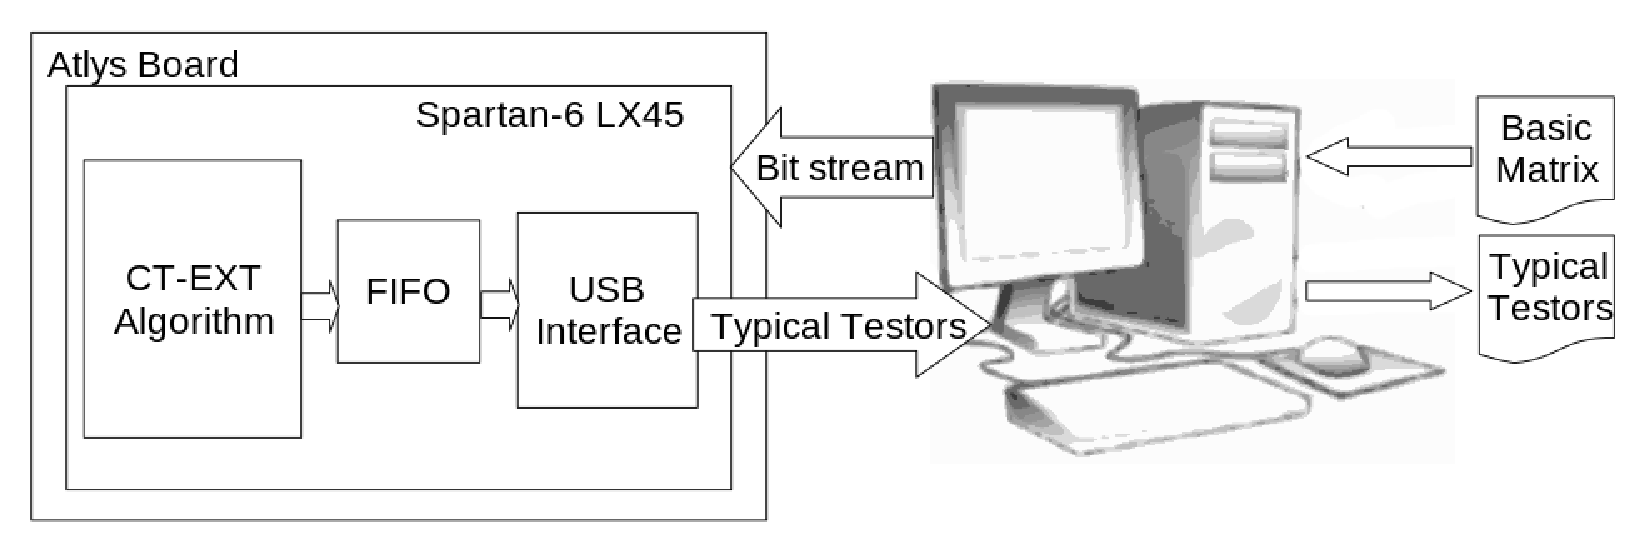
\includegraphics[width=13cm]{Arquitecture.eps}
    \end{center}
\caption{Proposed hardware-software platform.}
\label{figArq}
\end{figure}

\section{Hardware architecture}
\label{sect:4}

\begin{figure}[htb]
    \begin{center}
        %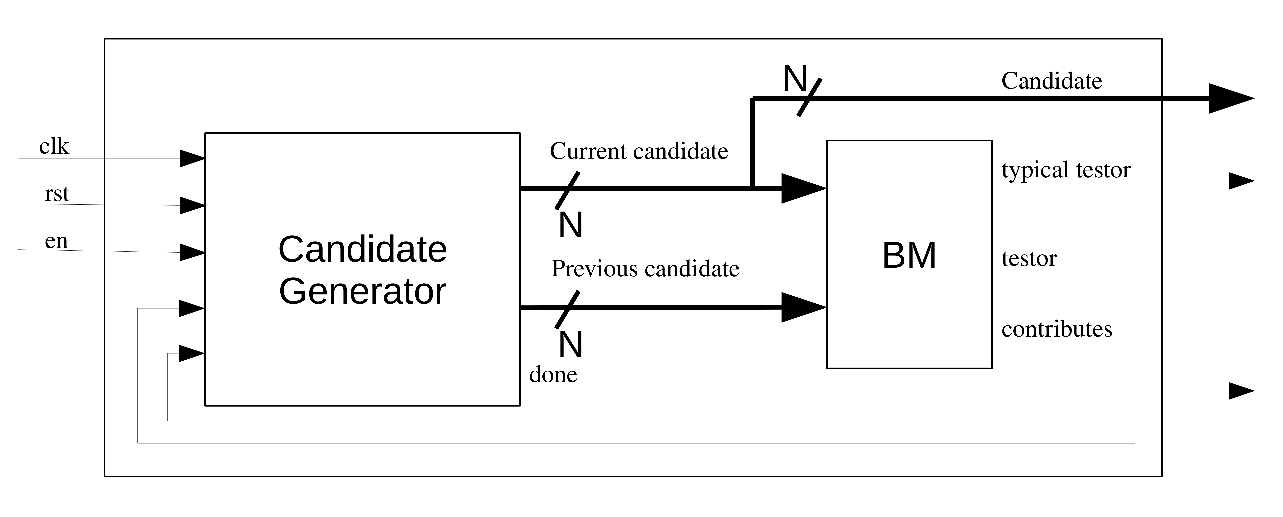
\includegraphics[width=13cm]{CT-ext_arq.eps}
    \end{center}
\caption{CT-EXT Architecture.}
\label{fig:3}
\end{figure}

The process of deciding if an $N$-tuple is a testor of $BM$ involves
comparing the candidate against each one of the $BM$'s rows. For
software-only implementations, this is a big disadvantage, in
particular for large matrices with many rows. The proposed hardware
architecture exploits the parallelism inherent in the CT-EXT algorithm
and evaluates whether a candidate is an irreducible testor or not in a single
clock cycle. It is composed by two main modules as seen in
Fig.\,\ref{fig:3}. 
%TODO change from here
The BM module stores the input matrix and
includes logic to decide if an $N$-tuple is a testor. The candidate
generator module produces the candidates ($N$-tuples) to be
evaluated by the BM module. In order to calculate the next candidate
according to the BT algorithm, the architecture feedbacks the
evaluation result of the previous candidate to the generator module,
this allows to drastically reduce the number of candidates tested
thus the number of iterations needed by the algorithm. At this
point, the architecture is able to obtain all testors of $BM$,
however since only irreducible testors are of interest, a final
hardware processing module eliminates most of the testors that are
not irreducible before sending the remaining testors to the software
for final processing. The dismiss module exploits the way
consecutive testors are obtained. If a testor is a superset of at
least one previous testor, it is not an irreducible testor, thus it
is eliminated. This final process does not introduce delays, thus
the architecture is still capable of evaluating a candidate in a
single clock cycle.

\begin{figure}[htb]
    \begin{center}
        %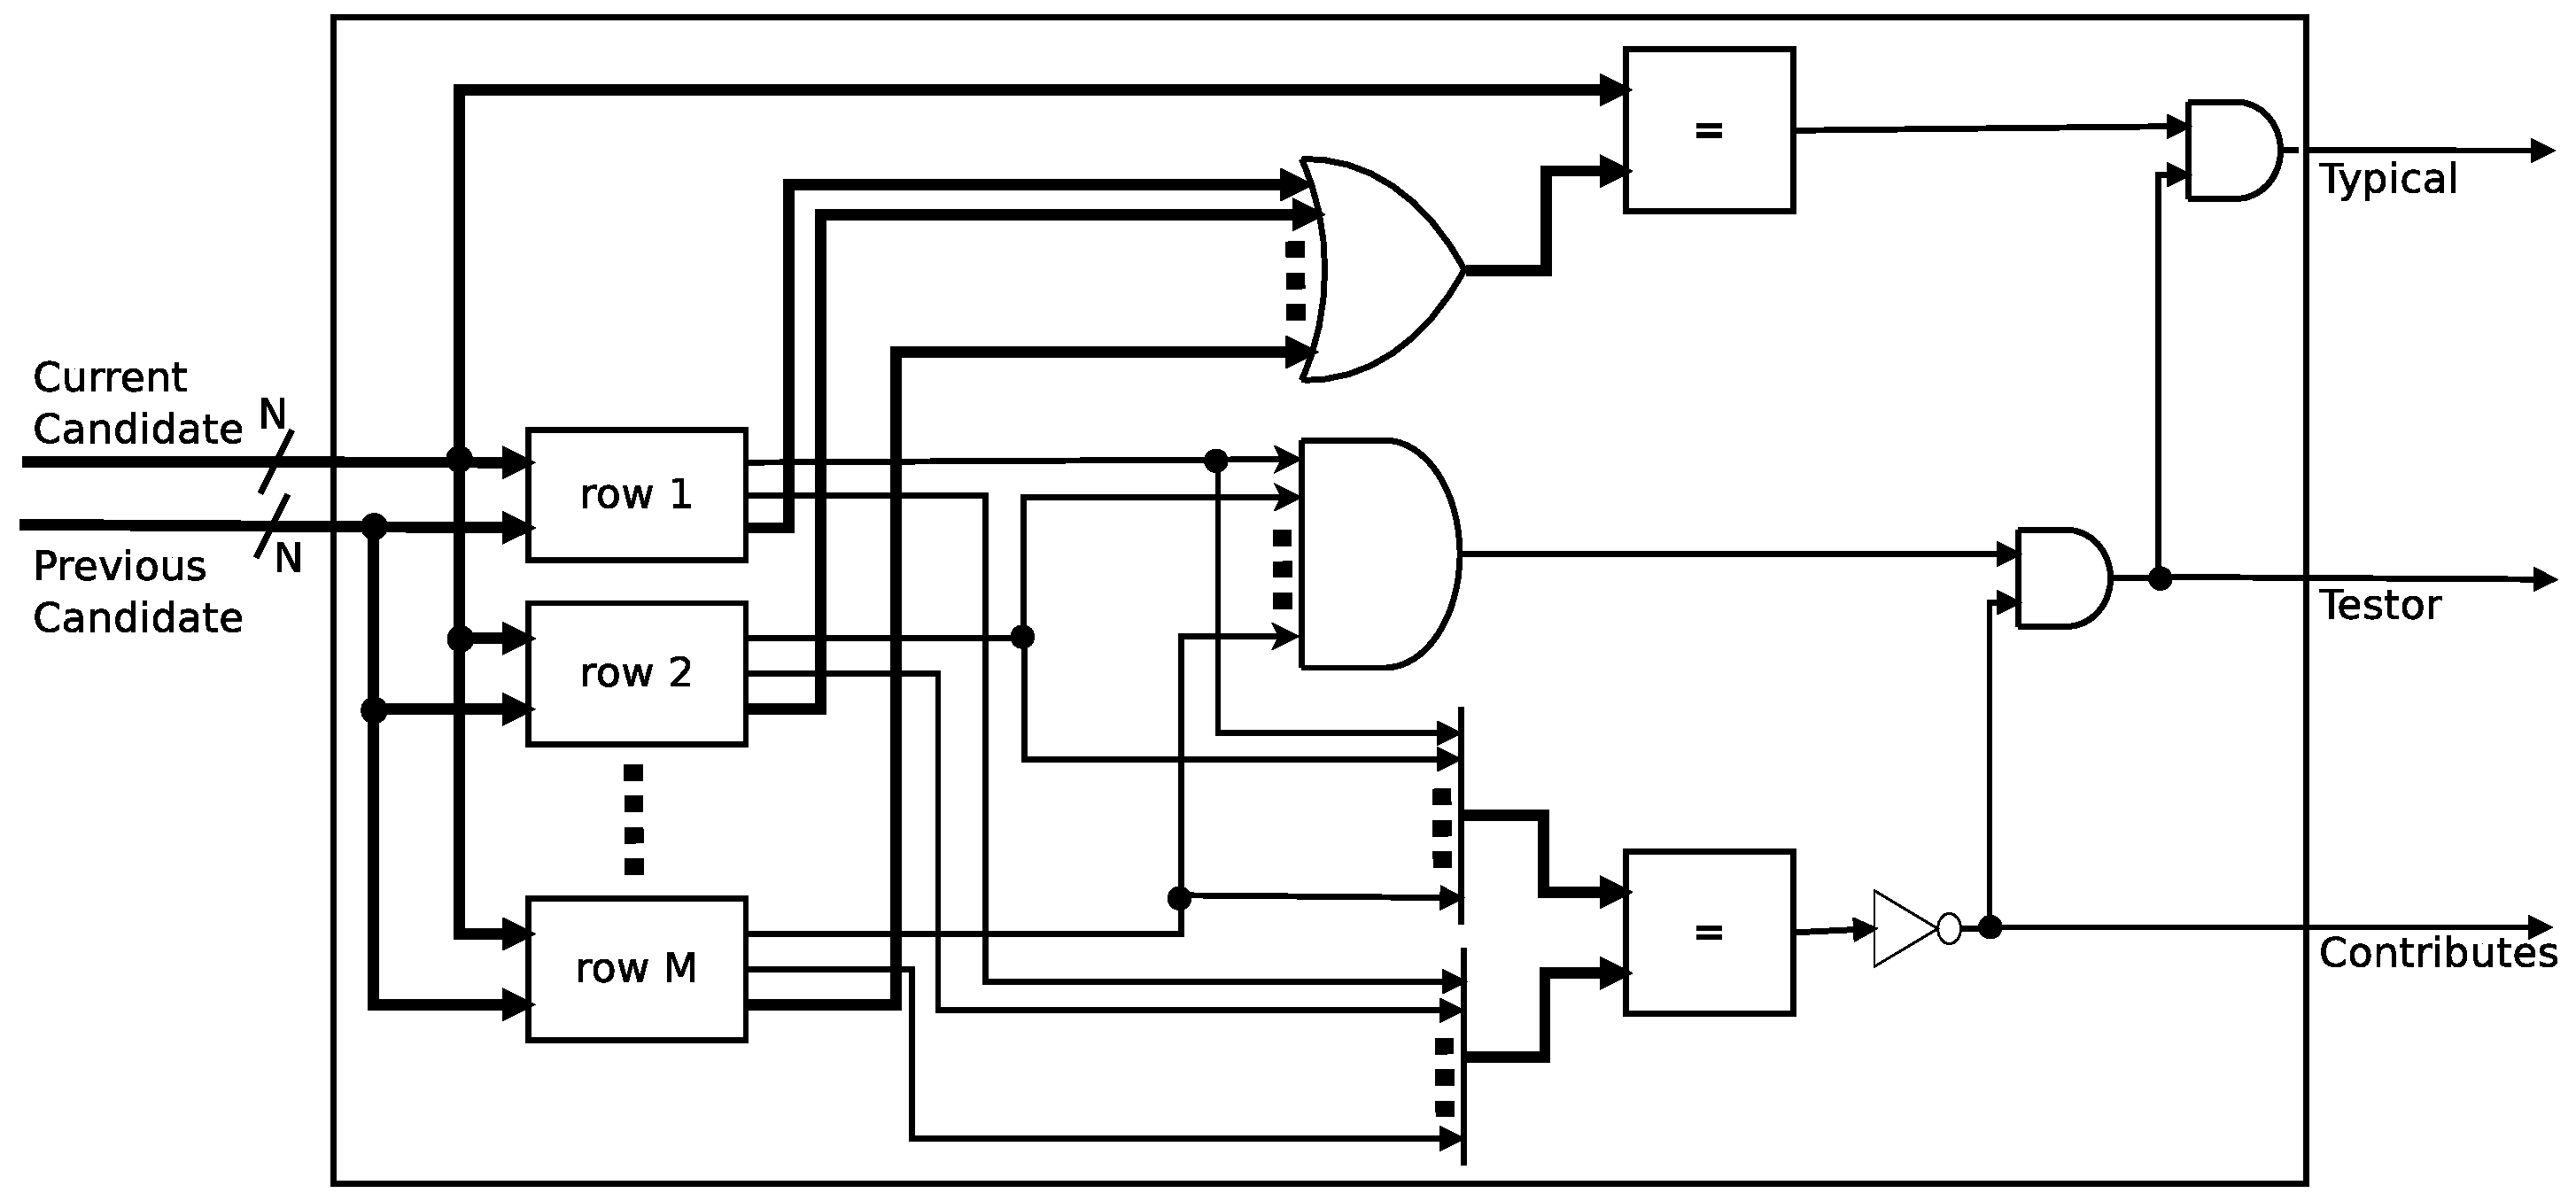
\includegraphics[height=6cm]{BM_module.eps}
    \end{center}
\caption{BM module.}
\label{fig:4}
\end{figure}

The BM module is composed of $M$ sub-modules named \textit{row~x}, as shown
in Fig.\,\ref{fig:4}. Each \textit{row~x} module contains a row ($N$ bits)
of the $BM$ matrix and logic to perform testor evaluation. To decide
if an $N$-tuple is a testor, a bitwise AND operation is performed
between the constant stored in each \textit{row~x} module and the current
candidate as shown in Fig.\,\ref{fig:row}. If at least one bit of the AND operation result is TRUE,
then the output \textit{Testor} of that particular \textit{row~x} sub-module
will be TRUE. The same operation is performed over the previous candidate.
If the count of rows asserting the output \textit{Testor} is different from
the those asserting the output \textit{Contributes} of that particular \textit{row~x} sub-module, 
then output \textit{Contributes} from the BM module is TRUE.
If the outputs of all  \textit{row~x} sub-modules are
TRUE, then the output \textit{Testor} of the BM module will be TRUE,
which means that the candidate is declared a testor of $BM$.

\begin{figure}[htb]
    \begin{center}
        %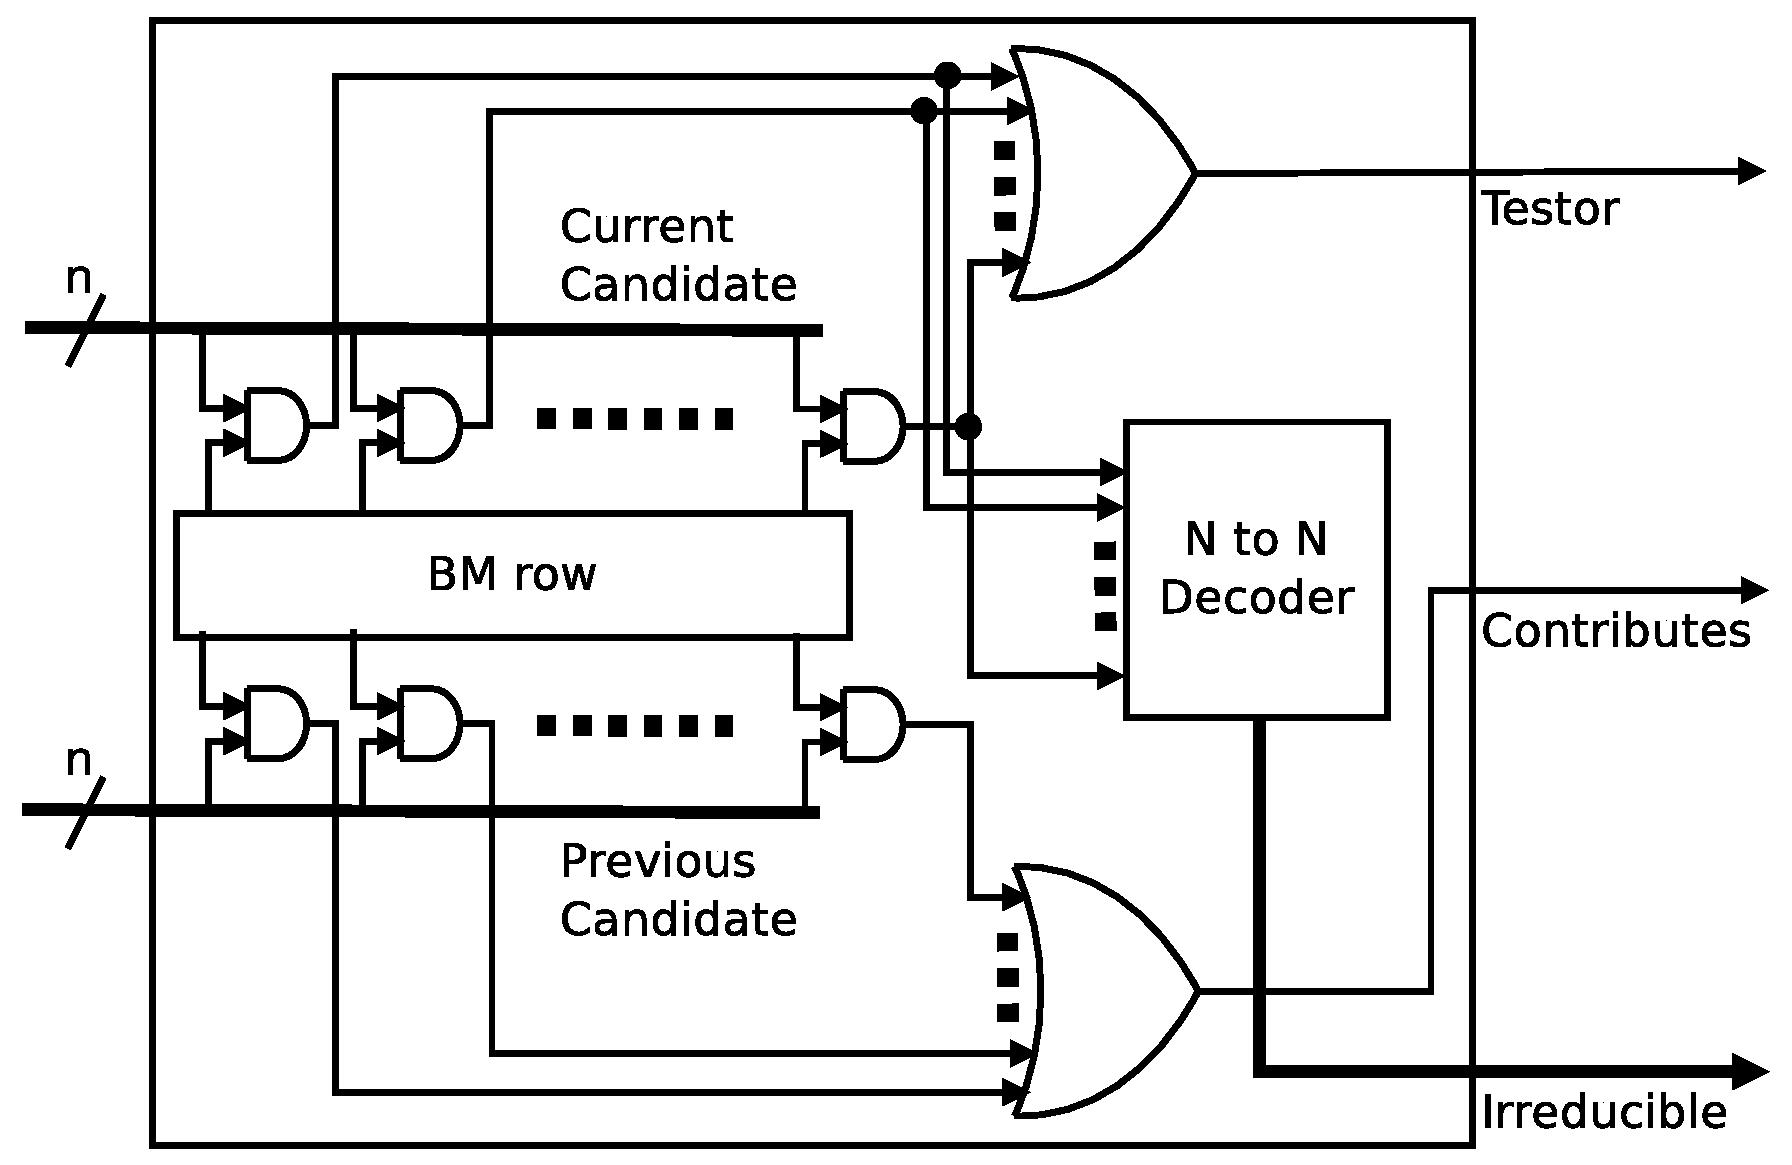
\includegraphics[height=6cm]{BM_row.eps}
    \end{center}
\caption{BM row.}
\label{fig:row}
\end{figure}

In order to check for irreducible condition of testors, the module \textit{N to N decoder}
receives as input the result of AND operation between the current candidate and the $BM$ row.
The output from module \textit{N to N decoder} repeats the input in case there is only one bit set
in it, and returns zero otherwise. For those rows with only one bit set after anded with candidate,
attribute in the position of setted bit is indispensable in case of candidate been a testor.
According to definition~\ref{def2}, every attribute in a testor should be indispensable to be an
irreducible testor. This idea is stated in definition~1 of \citep{R13}.

\setlength{\tabcolsep}{3pt}
\begin{table}[!htb]
    \begin{minipage}{.5\linewidth}
      \caption{Irreducible testor.}\label{table4}
      \centering
        \begin{tabular}{ ccccc|ccccc }
 			\hline                       
  			\multicolumn{5}{c|}{Cand. $(x_0 x_1)$} & 
  			\multicolumn{5}{c}{Decoder output} \\
  			\hline
  			%\multicolumn{5}{c|}{$x_0~x_3~x_4~x_1~x_2$}&\multicolumn{5}{c}{$x_0~x_3~x_4~x_1~x_2$}\\
  			$x_0$ & $x_3$ & $x_4$ & $x_1$ & $x_2$ &
  			$x_0$ & $x_3$ & $x_4$ & $x_1$ & $x_2$ \\
  			\hline
  			1 & 0 & 0 & 0 & 0 & 1 & 0 & 0 & 0 & 0\\
  			0 & 0 & 0 & 1 & 0 & 0 & 0 & 0 & 1 & 0\\
  			1 & 0 & 0 & 1 & 0 & 0 & 0 & 0 & 0 & 0\\
  			\hline  
  			\multicolumn{5}{c|}{Candidate $=$} & 1 & 0 & 0 & 1 & 0\\
  			\hline  
		\end{tabular}
	%\end{table}
	%\begin{table}[!htb]
    \end{minipage}%
    \begin{minipage}{.5\linewidth}
      \centering
        \caption{Non irreducible testor.}\label{table5}
        \begin{tabular}{ ccccc|ccccc }
 			\hline                       
  			\multicolumn{5}{c|}{Cand. $(x_0 x_4)$} & 
  			\multicolumn{5}{c}{Decoder output} \\
  			\hline
  			%\multicolumn{5}{c|}{$x_0~x_3~x_4~x_1~x_2$}&\multicolumn{5}{c}{$x_0~x_3~x_4~x_1~x_2$}\\
  			$x_0$ & $x_3$ & $x_4$ & $x_1$ & $x_2$ &
  			$x_0$ & $x_3$ & $x_4$ & $x_1$ & $x_2$ \\
  			\hline
  			1 & 0 & 1 & 0 & 0 & 0 & 0 & 0 & 0 & 0\\
  			0 & 0 & 1 & 0 & 0 & 0 & 0 & 1 & 0 & 0\\
  			1 & 0 & 1 & 0 & 0 & 0 & 0 & 0 & 0 & 0\\
  			\hline  
  			\multicolumn{5}{c|}{Candidate $\neq$} & 0 & 0 & 1 & 0 & 0\\
  			\hline  
		\end{tabular}
    \end{minipage} 
\end{table}


%When a candidate fails to be a testor of $BM$, the output $V$ of the
%BM module contains the value of the row closest to the top that
%caused the failure. If the candidate is declared as testor, the
%output $V$ is just ignored. The value of $V$ is obtained by using
%the output of a priority encoder as the $select$ signal of a
%multiplexer that can select among all the rows of BM. This is
%similar to having a read address in a register file to access the
%value stored in a particular row.

\begin{figure}[t]
    \begin{center}
        %\includegraphics[height=6cm]{Fig5.eps}
    \end{center}
\caption{Candidate Generator module.}
\label{fig:5}
\end{figure}

The candidate generator module uses the feedback from the BM module
to calculate the next candidate to be evaluated. As specified by the
BT algorithm, there are two ways of generating the next candidate
according to the evaluation result of the previous one. The
candidate generator module (Fig.\,\ref{fig:5}) consists of two
sub-modules, the first sub-module (jump\_1) generates the next
candidate when the previous one is a testor and the second
sub-module (jump\_2) generates the next candidate when the previous
one fails to be a testor. The next candidate is selected by a
multiplexer according to the evaluation result of the previous
candidate.

The jump\_1 sub-module uses a priority encoder to obtain the index,
$k$, of the last `1' in the previous candidate value. The next
candidate value is obtained by adding $2^{N-k}$ to the previous
candidate as indicated by the step 3 of the BT algorithm.

Besides the value of the previous candidate, the jump\_2 sub-module
uses an input $V$ that contains the value of the row of $BM$ that
caused the previous candidate not to be a testor. A priority decoder
obtains the index $k$ of the last `1' of $V$. By taking the value of
the previous candidate, the next candidate is obtained by letting
all bits to the left of the $k^{th}$ position unchanged, the bits to
the right are changed to `0', and the $k^{th}$ bit is set to `1'.
See step 4 of the algorithm.

\begin{figure}[b]
    \begin{center}
        %\includegraphics[width=13cm]{Fig6.eps}
    \end{center}
\caption{Dismiss Testors module.}
\label{fig:6}
\end{figure}

\begin{table*}[t]%[tpb]
\caption{Remaining testors using the Dismiss Testors module, with different amount of REG\_DT sub-modules.}
\label{table:4}
\begin{center}
    %\scalebox{.55}{
    \begin{tabular}{rrrrrrrrrr}\hline
           &  Received & \multicolumn{8}{c}{\bf \small Amount of registers in the dismiss testors module} \\ \cline{3-10}
        \raisebox{1.5ex}[0pt]{$BM$} & Testors & 8 & 16 & 32 & 64 & 128 & 256 & 512 & 1024 \\ \hline
        21 & 173,957 & 57,020 & 36,243 & 26,014 & 19,943 & 15,081 & 11,934 & 9,965 & 7,870 \\
        22 & 280,926 & 85,624 & 51,667 & 36,643 & 27,302 & 20,776 & 16,875 & 13,978 & 11,176 \\
        23 & 476,445 & 134,068 & 80,296 & 55,491 & 39,314 & 28,679 & 22,982 & 18,852 & 14,800 \\
        24 & 822,454 & 214,127 & 121,877 & 79,440 & 55,398 & 40,731 & 32,869 & 26,962 & 21,348 \\
        25 & 1,483,468 & 352,075 & 192,316 & 124,136 & 84,781 & 59,736 & 47,075 & 37,549 & 29,356 \\
        26 & 2,506,239 & 537,179 & 281,416 & 176,384 & 117,335 & 84,304 & 67,515 & 54,513 & 42,936 \\
        27 & 4,492,643 & 839,811 & 443,758 & 272,190 & 175,103 & 123,866 & 98,442 & 77,682 & 61,278 \\
        28 & 6,712,871 & 1,236,039 & 637,972 & 385,418 & 246,115 & 170,057 & 133,463 & 105,581 & 84,056 \\
        29 & 9,956,854 & 1,727,804 & 892,049 & 551,305 & 355,303 & 247,730 & 193,879 & 151,596 & 120,986 \\ \hline
    \end{tabular}%}
\end{center}
\end{table*}


The Dismiss Testors (DT) module (Fig.\,\ref{fig:6}) discards some
candidates that were evaluated as testors in the BM module, but they
are supersets of other testors, thus they are not irreducible
testors. The DT module has a predefined number of REG\_DT
sub-modules that store equal number of testors. These sub-modules
are initialized with the $N$-tuple $1\ldots11$. A new testor is
evaluated in each sub-module. If the input testor is a superset of
any of the stored ones, it must be disposed, else, it is sent to the
output $testor$ and furthermore, it is stored in the first REG\_DT
sub-module. Each time a new testor is stored, each REG\_DT
sub-module passes its value to the next one. As the number of
registers within the REG\_DT sub-modules is limited, a discarding
policy must be implemented to delete a testor once all sub-modules
are filled. Because the last testor is more likely to be a superset
of one or more of the previously generated testors, the selected
discarding policy consists in eliminating the oldest testor stored
within the DT module.

On each REG\_DT sub-module, a bitwise AND operation is performed
between the stored value in the register and the input $Candidate$.
The $N$-tuple stored is compared again, this time against the result
of the previous operation. If both are equal, it means that the
input testor is a superset of the stored one. The output of each
REG\_DT sub-module always takes the value stored in the register,
moving out this value to the next register in case of being
necessary.

The used prototyping kit allows partitioning the functionality of the application between software and
hardware effectively. It provides a set of functions that allows the user to communicate data between the
hardware architecture in the FPGA and the host application running on the PC using high level calls. An
interface core provided with the kit offers a communication mechanism to build a simplified interface for
connecting the user architecture in the FPGA to the PCI bus using a FIFO memory as buffer. This abstracts the
complexities of the communication process.  In turn, for the host application, a set of Application Program
Interfaces (APIs) provides functions for sending and receiving data from across the PCI \citep{R15}.

Table \ref{table:4} summarizes experiments made for deciding the
appropriate number of registers in the dismiss testors module. As
results show, the more REG\_DT sub-modules, the higher the
percentage of non irreducible testors eliminated. However, as the
number of REG\_DT sub-modules impacts directly on hardware
requirements, we concluded that 16 REG\_DT provide a good tradeoff
for two reasons: 1) the percentage of non irreducible testors
eliminated was always over 79\%; and 2) as shown in
Table\,\ref{table:7} (in Sect.\,\ref{sect:6}), the hardware
requirements are still modest when compared against the rest of the
architecture. This number of REG\_DT is used for all the
experiments.

\section{Software Description}
\label{sect:5}

The software component of the hardware-software platform works as an
interface between the user, the computer, and the FPGA board.
Fig\,\ref{fig:7} shows the user interface, which requests the
location of the input file containing the basic matrix, and allows
starting and stopping the irreducible testor computing process. The
input data file must be in plain text following the format shown in
Fig.\,\ref{fig:8}.

The process of deciding if a testor obtained by the architecture is
an irreducible testor by the host application is straightforward. It
consists in deciding for each new testor, if it is a superset of any
previously stored testor, which indicates that the new testor is not
an irreducible testor, and it must be discarded. This process starts
once the first testor is received by the host application, from that
moment until the last testor is received, both the hardware
architecture and the host application work alternately. Thus the
processing times reported in Table \ref{table:5} for the irreducible
testors processing is mostly the time spent by the hardware
architecture to produce the testors, including the time needed for
deciding which of the testors obtained by the architecture are
indeed irreducible testor. The platform is able to extract all
irreducible testors independently of the number of Reg\_DTs. The
purpose of the DT module is to reduce the number of testors sent to
the host application in order to avoid having a bottleneck in the
system. The amount of the reduction can be seen in table
\ref{table:4}.

The testor computing process begins when the user clicks the $Start$
button. First the basic matrix is read from the input file. Once the
matrix is loaded into the computer's memory, the basic matrix is
reorganized by swapping rows and columns in such a way the resulting
basic matrix is close to be a lower-left-triangular matrix, this
with the purpose of optimizing the jumps that BT algorithm performs.
Afterward, in order to complete the project files, three VHDL files
are generated and used to create a project for ISE (implementation
tool from Xilinx), which produces the programming file for the FPGA
device.

In the next stage, the interaction between hardware and software is
started. First, the board and the FPGA are located, then the device
is programmed with the bit-file obtained from the previous stage,
and both, the board and the device are initialized. Now, the
hardware architecture starts computing testors. Each testor is
temporally stored in a FIFO memory, when there are 512 elements in
the FIFO they are sent to the software through the PCI bus. The
software stores the incoming testor set into a buffer. When the
buffer is full, the hardware is paused while a selection process
empties the buffer by choosing and storing only irreducible testors.
After this, the hardware architecture and the software alternate
until the last candidate is verified.

\begin{figure}[t]
    \begin{center}
        %\includegraphics[height=6cm]{Fig7.eps}
    \end{center}
\caption{User interface for BT hardware-software platform.}
\label{fig:7}
\end{figure}

\begin{figure}[t]
    \begin{center}
       % \includegraphics[height=2.8cm]{Fig8.eps}
    \end{center}
\caption{$BM$ input file format.}
\label{fig:8}
\end{figure}

\section{Evaluation}
\label{sect:6}

\begin{table*}[t]%[tpb]
    \caption{Processing time in seconds (broken down for each stage) for 45X100 low, medium and high density matrices.}
    \label{table:5}
    \begin{center}
        %\scalebox{.7}{
        \begin{tabular}{ccccccc} \cline{2-7}
             & \multicolumn{2}{c}{\bf Low Density} & \multicolumn{2}{c}{\bf Medium Density} & \multicolumn{2}{c}{\bf High Density} \\ \hline
            Stages & HW/SW & SW-O & HW/SW & SW-O & HW/SW & SW-O \\ \hline
            Load BM & 0.031 & 0.031 & 0.031 & 0.031 & 0.032 & 0.031 \\
            BM arrangement & 0.281 & 0.281 & 0.281 & 0.024 & 0.282 & 0.01 \\
            Files creation & 0.032 & N/A \footnote[1]{Not Applicable} & 0.031 & N/A\footnote[1]{Not Applicable} & 0.046 & N/A\footnote[1]{Not Applicable} \\
            Synthesis & 691 & N/A\footnote[1]{Not Applicable} & 1,032 & N/A\footnote[1]{Not Applicable} & 930 & N/A\footnote[1]{Not Applicable} \\
            IT\footnote[2]{Irreducible testors.} computing & 316 & 170,830 & 1,303 & 51,777 & 8 & 0.06 \\ \hline
            TOTAL & 1,008 & 170,831 & 2,336 & 51,778 & 939 & 0.11 \\ \hline
        \end{tabular}%}
    \end{center}
\end{table*}

In order to show the performance of the proposed hardware-software
platform, it was compared against a software-only implementation of
the BT algorithm. For experimentation purposes, three kinds of basic
matrices were randomly generated. Each type containing different
amount of 1's per row:

\begin{enumerate}
\renewcommand{\labelenumi}{\arabic{enumi})}
    \item High density matrices: between 90\% and 98\%.
    \item Low density matrices: between 4\% and 12\%.
    \item Medium density matrices: between 47\% and 53\%.
\end{enumerate}

\footnotetext[1]{Not Applicable}
\footnotetext[2]{Irreducible Testors}

High density matrices represent datasets with well separated
classes, so it is very easy to find out subsets of features that
allow differentiating objects from different classes; in consequence
it is easy to compute all irreducible testors. On the other hand,
low density matrices represent datasets where objects from different
classes are very similar, which results in a low amount of 1's;
therefore it is difficult to find a feature subset that allows to
distinguish between objects belonging to different classes and
computing all irreducible testors would be more difficult. Medium
density matrices contain a balanced amount of 1's and 0's, and they
come from datasets where the classes are not well separated, but
there still be enough difference between objects from different
classes. These are difficult matrices for computing all irreducible
testors, and in practice, most of the interesting pattern
recognition problems produce this kind of matrices.

Several basic matrices of different sizes were randomly generated
for each density, from 35 to 50 columns and all of them with 100
rows. On the hardware-software platform the runtimes for the
following stages: load basic matrix to memory, matrix arrangement,
project files creation, synthesis of ISE project, and irreducible
testor computing (with a hardware frequency of 40MHz), were
measured. Figs.\,\ref{fig:9},\,\ref{fig:10} and \,\ref{fig:11} show
graphs of the whole processing time for high, medium and low density
matrices respectively. In these graphs, it is possible to see that
the proposed platform obtains better performance than the
software-only implementation of BT for low and medium density
matrices. For high density matrices the software-only implementation
required less time, because computing irreducible testors is very
easy for this kind of matrices, and the synthesis time required for
the proposed platform is much higher than the irreducible testor
computing time.

The processing time $t$, of the last stage of the proposed platform,
for a specific matrix is given by:

\begin{equation}
    \label{eq:1}
    t = \left( \frac{2^{N}}{f} \right) \left( \frac{c}{100} \right)
\end{equation}

\begin{figure}[t]
    \begin{center}
       % \includegraphics[width=13.0cm,height=6cm]{Fig9.eps}
%        \includegraphics{Fig9.eps}
    \end{center}
\caption{Whole processing time in hours for high density matrices.}
\label{fig:9}
\end{figure}

\begin{figure}[t]
    \begin{center}
       % \includegraphics[width=13cm,height=6.0cm]{Fig10.eps}
%        \includegraphics{Fig10.eps}
    \end{center}
\caption{Whole processing time in hours for medium density matrices.}
\label{fig:10}
\end{figure}

\begin{figure}[t]
    \begin{center}
        %\includegraphics[width=13cm,height=6.0cm]{Fig11.eps}
%        \includegraphics{Fig11.eps}
    \end{center}
\caption{$BM$ Whole processing time in hours for low density matrices.}
\label{fig:11}
\end{figure}


\begin{table}[t]%[tpb]
\caption{Synthesis summary of FPGA Resources utilization a operating
frequency for the architecture targeted for a Virtex-II XC2V3000
FPGA device (N = 100, M = 325).} \label{table:6}
\begin{center}
    \begin{tabular}{ccccc}   \hline
        Number of Slices & 11,137 (77\%)  \\
        Number of 4-input LUTs & 2,484 (8\%) \\
        Number of Flip-Flops & 2,1262 (74\%) \\
        Maximum clock frequency & 55.510 MHz \\ \hline
    \end{tabular}
\end{center}
\end{table}


\begin{table*}[t]%[tpb]
\caption{FPGA Resource utilization for Virtex II XC2V3000 for $N=50$ and $M=100$ (Whole
architecture vs Dismis testors module).}
 \label{table:7}
\begin{center}
    %\scalebox{.68}{
    \begin{tabular}{ccccccc} \cline{2-7}
         & \multicolumn{2}{c}{\bf8 REG\_DT} & \multicolumn{2}{c}{\bf16 REG\_DT} & \multicolumn{2}{c}{\bf32 REG\_DT} \\ \hline
         & Whole & Dismiss & Whole & Dismiss & Whole & Dismiss \\
        \raisebox{1.5ex}[0pt]{\bf Resources} & architecture & Testors & architecture & Testors & architecture & Testors \\ \hline
        Slices & 2365 & 338 & 2676 & 679 & 3331 & 1342 \\
        Flip-flops & 1024 & 400 & 1451 & 800 & 2236 & 1600 \\
        LUTs & 4256 & 258 & 4472 & 472 & 4871 & 892 \\ \hline
    \end{tabular}%}
\end{center}
\end{table*}

where $f$ is the clock frequency of the architecture and $c$ is the
percentage of candidates tested. Note that the value of $c$ is data
dependent, i.e. it varies for each basic matrix, $BM$.

It is important to notice that the processing time for computing
irreducible testors does not only depend on the size and density of
the $BM$, but also on the distribution of 0's and 1's inside the
matrix. This assertion can be appreciated in points 43 to 45 of
Fig\,\ref{fig:11}.

Table\,\ref{table:5} shows the processing time for each stage of the data flow, for 45X100 low, medium, and
high density matrices. This table shows that the proposed platform allows running BT 169 times faster that
the software-only implementation, for a 45X100 low density matrix and 22 times faster for the medium density
matrix of the same size. Moreover, taking into account only the last stage of the data flow, the improvement
over the software is 540X for the low density matrix and 39X for the medium density one. The only type of
matrices where the proposed platform does not perform better that the software-only BT implementation was the
high density ones, this is because of computing irreducible testors is very fast for this kind of matrices.
The software-only implementation of BT was executed on a PC with an Intel Centrino Duo processor running at
1.6GHz, with 1024 MB of RAM.

The proposed platform has been designed to process variable sizes of the $BM$ matrix. The maximum size of the
matrix that can be implemented is only limited by the available resources on the specific FPGA board. For
example, for the Virtex-II XC2V3000 from Xilinx\cite{R14} embedded on an XtremeDSP board \citep{R15}, the
biggest medium density matrix that can fit into the FPGA is about 100X325. Table\,\ref{table:6} summarizes
the resource utilization for this matrix.

Finally, Table\,\ref{table:7} summarizes the resource utilization
for a 50X100 matrix for different buffer sizes on the Dismiss Testor
module, all for the same device. Although 8 and 32 are good choices,
16 results in a better trade-off between resource utilization (small
when compared against the whole architecture), and the non
irreducible testors eliminated (always over 79\%, as
Table\,\ref{table:4} shows).

\section{Discussion}
\label{sect:7}

The proposed hardware-software platform provides higher processing
performance than the software-only implementation of the BT
algorithm for two of the three kinds of matrices used in the
experimentation. This behavior is possible because the hardware
component of the proposed platform is capable of testing if an
$N$-tuple is a testor of a $BM$ in a single clock cycle,
independently of the number of columns and rows, whereas
software-only implementation processing time will significantly
increase for matrices with a large number of rows.

Moreover, the performance improvement is directly related to the
percentage of candidates tested ($c$), which heavily depends on
density and distribution of the values into the $BM$ matrix. Proofs
for this dependence are the resulting processing times of high
density matrices. This kind of matrices has a high amount of 1's,
thus there are low chances to find a row with only 0's when an
$N$-tuple is evaluated, which results in a great reduction in the
number of operations made by the BT algorithm. This occurs in the
software-only as well as in the hardware-software implementations,
but the proposed platform also needs to synthesize the specific
architecture. Therefore, the best choice for computing all
irreducible testors for high density matrices is the software-only
implementation of BT algorithm. However, most of the real world
pattern recognition problems produce medium density matrices, where
using the proposed platform is the best choice for computing all
irreducible testors.

Experiment results show that the proposed platform allows computing
irreducible testors faster than the software-only implementation of
the BT algorithm, with improvements in the range of 2 orders of
magnitude. However, for very large real data this improvement could
be significantly higher.

\section{Conclusions}
\label{sect:8}

The high performance of the proposed platform is feasible due to the
high level of parallelism implicit in the BT algorithm which can be
efficiently implemented on an FPGA. The proposed architecture is
capable of evaluating a testor candidate in a single clock cycle for
any $BM$ matrix, regardless of the number of columns and rows, the
only limitation being the size of the FPGA device used. The
architecture provides a good trade-off between performance and
hardware resource utilization and it is suitable to be used as a
high performance processing module in a hardware-in-the-loop
approach\cite{R16}.

Even though the proposed architecture offers an improvement compared
with a previously reported hardware implementation, further
improvements, such as testing two or more candidates per iteration,
are still possible. Also, because resource requirements are
relatively small, a scheme where the processing core can be
replicated will also be explored; this will effectively reduce the
processing time, in proportion to the number of processing cores
that can be accommodated on the FPGA device.


%% The Appendices part is started with the command \appendix;
%% appendix sections are then done as normal sections
%% \appendix

%% \section{}
%% \label{}

%% References
%%
%% Following citation commands can be used in the body text:
%%
%%  \citet{key}  ==>>  Jones et al. (1990)
%%  \citep{key}  ==>>  (Jones et al., 1990)
%%
%% Multiple citations as normal:
%% \citep{key1,key2}         ==>> (Jones et al., 1990; Smith, 1989)
%%                            or  (Jones et al., 1990, 1991)
%%                            or  (Jones et al., 1990a,b)
%% \cite{key} is the equivalent of \citet{key} in author-year mode
%%
%% Full author lists may be forced with \citet* or \citep*, e.g.
%%   \citep*{key}            ==>> (Jones, Baker, and Williams, 1990)
%%
%% Optional notes as:
%%   \citep[chap. 2]{key}    ==>> (Jones et al., 1990, chap. 2)
%%   \citep[e.g.,][]{key}    ==>> (e.g., Jones et al., 1990)
%%   \citep[see][pg. 34]{key}==>> (see Jones et al., 1990, pg. 34)
%%  (Note: in standard LaTeX, only one note is allowed, after the ref.
%%   Here, one note is like the standard, two make pre- and post-notes.)
%%
%%   \citealt{key}          ==>> Jones et al. 1990
%%   \citealt*{key}         ==>> Jones, Baker, and Williams 1990
%%   \citealp{key}          ==>> Jones et al., 1990
%%   \citealp*{key}         ==>> Jones, Baker, and Williams, 1990
%%
%% Additional citation possibilities
%%   \citeauthor{key}       ==>> Jones et al.
%%   \citeauthor*{key}      ==>> Jones, Baker, and Williams
%%   \citeyear{key}         ==>> 1990
%%   \citeyearpar{key}      ==>> (1990)
%%   \citetext{priv. comm.} ==>> (priv. comm.)
%%   \citenum{key}          ==>> 11 [non-superscripted]
%% Note: full author lists depends on whether the bib style supports them;
%%       if not, the abbreviated list is printed even when full requested.
%%
%% For names like della Robbia at the start of a sentence, use
%%   \Citet{dRob98}         ==>> Della Robbia (1998)
%%   \Citep{dRob98}         ==>> (Della Robbia, 1998)
%%   \Citeauthor{dRob98}    ==>> Della Robbia


%% References with bibTeX database:

\bibliographystyle{elsarticle-harv}
%%\bibliography{<your-bib-database>}

%% Authors are advised to submit their bibtex database files. They are
%% requested to list a bibtex style file in the manuscript if they do
%% not want to use elsarticle-harv.bst.

%% References without bibTeX database:

\begin{thebibliography}{00}

\bibitem[Al-ani (2009)]{R17} Al-Ani, A. (2009). A dependency-based search strategy for feature selection Expert Systems with Applications, 36, 12392-12398.
\bibitem[Asaithambi et al. (2004)]{R6}Asaithambi, A. and Valev, A. (2004). Construction of all non-reductible descriptors. Pattern Recognition, 37, 1817-1823.
\bibitem[Chen et al. (2008)]{R18}Chen, w. S., Tseng, S. S. and Hong, T. P. (2008). An efficient bit-based feature selection method. Expert Systems with Applications, 34, 2858-2869.
\bibitem[Cumplido et al. (2006)]{R10} Cumplido, R., Carrasco, A. and Feregrino, C. (2006). On the Design and Implementation of a High Performance Configurable Architecture for Testor Identification. Lectures Notes on Computer Science, 4225, 665-673.
\bibitem[Djukova (2005)]{R8}Djukova, E. V. (2005). On the number of irreducible coverings of an integer Matrix. Computational Mathematics and Mathematical Physics, 45, 903-908.
\bibitem[Dmitriev et al. (1966)]{R12} Dmitriev, A. N.,  Zhuravlev, Y. I. and Krendeliev, F. P. (1966). About Mathematical Principles of Objects and Phenomena Classification. Diskretni Analiz, 7, 3-17.
\bibitem[G\'omez (2001)]{R16}G\'omez, M. (2001). Hardware-in-the-Loop Simulation. Embedded Systems Programming, 14, 38-49.
\bibitem[Guyon at el. (2003)]{R4}Guyon, I. and Elisseeff, A. (2003). An introduction to variable and feature selection. Journal of Machine Learning Research, 3, 1157-1182.
\bibitem[Jain et al. (1997)]{R3}Jain, A. and Zongker, D. (1997). Feature Selection: Evaluation, Application, and Small Sample Performance. IEEE Transactions on Pattern Analysis and Machine Intelligence, 9, 153-158.
\bibitem[Kudryavtsev (2006)]{R9}Kudryavtsev, V. B. (2006). Test recognition theory. Discrete Applied Mathematics, 16, 319-350.
\bibitem[Kwan et al. (2002)]{R2}Kwan, N. and Choi, C. H. (2002). Input feature selection for classification problems. IEEE Transactions on Neural Networks, 13, 143-159.
\bibitem[Lazo-Cort\'es et al.(2001)]{R1}Lazo-Cort\'es, M., Ruiz-shulcloper, J., and Alba-cabrera, E. (2001). An Overview of the Evolution of the Concept of Testor. Pattern Recognition, 34, 753-762.
\bibitem[Liu et al. (1998)]{R19} Liu, H. and Setiono, R. (1998).Some issues on scalable feature selection. Expert Systems with Applications, 15, 333-339.
\bibitem[Mart\'inez-Trinidad et al. (2001)]{R5}Mart\'inez-Trinidad, J.F. and Guzm\'an-Arenas, A. (2001). ``The Logical Combinatorial Approach to Pattern Recognition an Overview through Selected Works. Pattern Recognition, 34, 741-751.
\bibitem[Rojas et al. (2007)]{R11}Rojas, A., Cumplido, R., Carrasco-Ochoa, J. A., Feregrino, C. and Mart�nez-Trinidad, J. f. (2007). FPGA Based Architecture for Computing Testors. Lectures Notes on Computer Science, 4881, 188-197.
\bibitem[Rojas et al. (2012)]{R21}Rojas, A., Cumplido, R., Carrasco-Ochoa, J. A., Feregrino, C. and Mart�nez-Trinidad, J. f. (2012). Hardware-software platform for computing irreducible testors. Expert Systems with Applications, 39, 2203 - 2210.
\bibitem[S\'anchez-D\'iaz et al. (2002)]{R13}S\'anchez-D\'iaz, G. and Lazo-Cort\'es, M. (2002). Modifying BT Algorithm for Improving its Runtimes. Revista Ciencias Matem\'aticas, 20, 129-136.
\bibitem[S\'anchez-D\'iaz et al. (2007)]{R22}S\'anchez-D\'iaz, G. and Lazo-Cort\'es, M. (2007). CT-EXT: An Algorithm for Computing Typical Testor Set. Lecture Notes in Computer Science, 4756, 506-514.
\bibitem[S\'anchez-D\'iaz et al. (2010)]{R23}S\'anchez-D\'iaz, G., Piza-Davila, I, Lazo-Cort\'es, M, 
Mora-Gonz\'alez, M and Salinas-Luna, J. (2010). A Fast Implementation of the CT-EXT Algorithm for the Testor Property Identification. Lecture Notes in Computer Science, 6438, 92-103.
\bibitem[Valev et al. (2004)]{R7}Valev, V. and Sankur, B. (2004). Generalized non-reducible descriptors. Pattern Recognition, 37, 1809-1815.
%TODO change these bellow for corect ones
\bibitem[Xilinx (2007)]{R14}Virtex-II Pro Data Sheet Version 4.7. Xilinx Inc.
\bibitem[Xilinx (2003)]{R15}XtremeDSP Development Kit Pro User Guide Version 1.0. Xilinx Inc.


%% \bibitem must have one of the following forms:
%%   \bibitem[Jones et al.(1990)]{key}...
%%   \bibitem[Jones et al.(1990)Jones, Baker, and Williams]{key}...
%%   \bibitem[Jones et al., 1990]{key}...
%%   \bibitem[\protect\citeauthoryear{Jones, Baker, and Williams}{Jones
%%       et al.}{1990}]{key}...
%%   \bibitem[\protect\citeauthoryear{Jones et al.}{1990}]{key}...
%%   \bibitem[\protect\astroncite{Jones et al.}{1990}]{key}...
%%   \bibitem[\protect\citename{Jones et al., }1990]{key}...
%%   \harvarditem[Jones et al.]{Jones, Baker, and Williams}{1990}{key}...
%%

% \bibitem[ ()]{}

\end{thebibliography}

\end{document}

%%
%% End of file `elsarticle-template-harv.tex'.
